\section*{Дифференциальные уравнения. Часть 2.}
\section*{Глава 6. Теория устойчивости}

\section{Введение}

\begin{center}
	\begin{tikzpicture}
		\node (napoleon) at (0,0) {Наполеон Бонапарт};
		\node (laplace) at (8,0) {Пьер Симон Лаплас};
		\draw[->, thick] (napoleon) -- node[above] {\small министр} node[below] {\small внутренних дел} (laplace);
	\end{tikzpicture}
\end{center}

\begin{itemize}
	\item Закон эволюции Вселенной (дифференц. ур-ния) \\
	+ Начальные краевые условия \\
	$\rbrace$ возможность предсказывать будущее?
\end{itemize}

\begin{center}
	\begin{tikzpicture}
		\node[align=center] (start) at (0,0) {Когда решения \\ ДУ будут \\ устойчивыми?};
		\node[align=center] (middle) at (5,0) {Решения дифференц. \\ ур-ний могут быть \\ неустойчивыми:};
		\node[align=center] (fail) at (10,0) {Провальная идея};
		
		\draw[->, thick] (fail) -- (middle);
		\draw[->, thick] (middle) -- (start);
		\draw[->, thick] (start) -- node[right] {1892 г. Ляпунов} (0,-2);
		
		\node[text width=6cm, align=center, font=\small] at (5,-2) {малое изменение данных может приводить к значительным изменениям решения};
	\end{tikzpicture}
\end{center}

\section{Устойчивость по Ляпунову. Основные понятия}

\begin{itemize}
	\item Рассмотрим систему $n$ дифференциальных уравнений относительно $n$ функций $x_1(t), x_2(t), \dots, x_n(t)$, записанную в нормальной форме Коши:
\end{itemize}

\begin{equation} \label{eq:197}
	\begin{cases}
		\dv{x_1}{t} = f_1(x_1, x_2, \dots, x_n, t) \\
		\dots \dots \dots \dots \\
		\dv{x_n}{t} = f_n(x_1, x_2, \dots, x_n, t)
	\end{cases}
	\quad (197)
\end{equation}

Запишем систему в сокращенной форме:
\begin{equation} \label{eq:198}
	\dv{x_i}{t} = f_i(x_1, x_2, \dots, x_n, t), \quad \text{где } i=1, 2, \dots, n \quad (198)
\end{equation}

Здесь $f_i$ -- некоторые заданные функции $(n+1)$-ой переменной.
$\exists$ функции $f_i$ таковы, что выполнены условия аналога теоремы Пикара для систем дифференциальных ур-ний. Такой выбор функции обеспечит единственность решения задачи Коши. Зададим некоторые начальные условия: $\left. x_i \right|_{t_0} = \varphi_{i0}$, $i=1, 2, \dots, n$. Они порождают решения $x_i(t) = \varphi_i(t)$.

Если изменить начальные условия, то решение системы изменится. Решение будет устойчивым, если при малых изменениях начальных условий оно меняется мало.

\begin{nb}
	1892 год. Ляпунов. Докторская диссертация <<Общая задача об устойчивости движения>>.
\end{nb}

\begin{definition}{Устойчивость по Ляпунову}{lyapunov_stability}
	Пусть $\varphi_i(t), i=1,2,\dots,n$ -- решение системы \eqref{eq:198}, удовлетворяющее начальным условиям $y_i(t_0)=\varphi_{i0}, i=1,2,\dots,n$. Это решение называется \textbf{устойчивым} по Ляпунову при $t \to \infty$, если для любого $\varepsilon > 0$ существует $\delta(\varepsilon) > 0$ такое, что начальные условия которого отличаются от $\varphi_i(t_0)$ меньше, чем на $\delta$:
	\begin{equation} \label{eq:199}
		|x_i(t_0) - \varphi_i(t_0)| < \delta, \quad i=1,2,\dots,n \quad (199)
	\end{equation}
	значения ф-ий будут отличаться от $\varphi_i(t)$ меньше, чем на $\varepsilon$:
	\begin{equation} \label{eq:200}
		|x_i(t) - \varphi_i(t)| < \varepsilon, \quad i=1,2,\dots,n \quad (200)
	\end{equation}
	для всех $t \ge t_0$.
\end{definition}

Если при сколь угодно малом $\delta > 0$ хотя бы для одного решения $x_i(t), i=1,2,\dots,n$ неравенства \eqref{eq:200} не выполняются, то решение $\varphi_i(t)$ называется \textbf{неустойчивым}.

\begin{definition}{Асимптотическая устойчивость}{asymp_stability}
	Если кроме выполнения неравенств \eqref{eq:200} при условии \eqref{eq:199} выполняется также условие
	\begin{equation} \label{eq:201}
		\lim_{t \to \infty} |x_i(t) - \varphi_i(t)| = 0, \quad i=1,2,\dots,n \quad (201)
	\end{equation}
	то решение $\varphi_i(t), i=1,2,\dots,n$ называется \textbf{асимптотически устойчивым}.
\end{definition}

Из асимптотической устойчивости решения следует просто устойчивость. Но \textbf{НЕ} наоборот.

\subsection*{Устойчивость решения $x=\varphi(t)$}
В системе ур-ний \eqref{eq:198}: $n=1, t_0 > 1$.

\begin{center}
	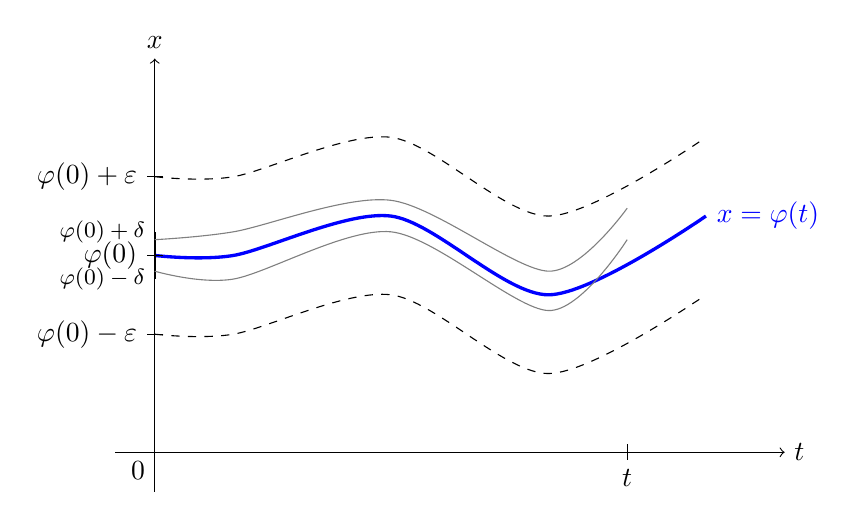
\begin{tikzpicture}
		% Axes
		\draw[->] (-0.5, 0) -- (8, 0) node[right] {$t$};
		\draw[->] (0, -0.5) -- (0, 5) node[above] {$x$};
		\node at (0,0) [below left] {$0$};
		
		% Coordinates
		\coordinate (t0) at (1, 2.5);
		\coordinate (tend) at (7, 2.5);
		
		% Main solution phi(t)
		\draw[very thick, blue] plot [smooth] coordinates {(0,2.5) (1,2.5) (3, 3) (5, 2) (7, 3)} node[right] {$x=\varphi(t)$};
		
		% Epsilon tube boundaries
		\draw[dashed] plot [smooth] coordinates {(0,3.5) (1,3.5) (3, 4) (5, 3) (7, 4)};
		\draw[dashed] plot [smooth] coordinates {(0,1.5) (1,1.5) (3, 2) (5, 1) (7, 2)};
		
		% Labels on y-axis
		\draw (0.1, 3.5) -- (-0.1, 3.5) node[left] {$\varphi(0)+\varepsilon$};
		\draw (0.1, 1.5) -- (-0.1, 1.5) node[left] {$\varphi(0)-\varepsilon$};
		\draw (0.1, 2.5) -- (-0.1, 2.5) node[left] {$\varphi(0)$};
		
		% Delta interval
		\draw[thick] (0, 2.2) -- (0, 2.8);
		\node[left, font=\footnotesize] at (0, 2.8) {$\varphi(0)+\delta$};
		\node[left, font=\footnotesize] at (0, 2.2) {$\varphi(0)-\delta$};
		
		% Another solution inside the tube
		\draw[gray] plot [smooth] coordinates {(0,2.7) (1,2.8) (3, 3.2) (5, 2.3) (6, 3.1)};
		\draw[gray] plot [smooth] coordinates {(0,2.3) (1,2.2) (3, 2.8) (5, 1.8) (6, 2.7)};
		
		% Time label
		\draw (6, 0.1) -- (6, -0.1) node[below] {$t$};
		
	\end{tikzpicture}
\end{center}

Если начальные данные не выходят за пределы интервала $(\varphi(0)-\delta, \varphi(0)+\delta)$, то решение во все моменты времени $t$ будет находиться внутри коридора $(\varphi(t)-\varepsilon, \varphi(t)+\varepsilon)$.

Исследовать произвольное решение на устойчивость часто бывает неудобно. Вместо этого можно исследовать некоторое конкретное решение. Самый простой путь --- рассмотреть нулевое решение. Попробуем переформулировать задачу.
Исследовать на устойчивость решения решения $\varphi_i(t), i=1,2,\dots,n$, устойчивость нулевого (тривиального) решения $x_i \equiv 0$ некоторой системы, аналогичной системе \eqref{eq:198}:
\begin{equation} \label{eq:202}
	\dv{x_i}{t} = F_i(x_1, x_2, \dots, x_n, t), \quad i=1,2,\dots,n \quad (202)
\end{equation}
где $F_i(0, 0, \dots, 0, t) \equiv 0, i=1,2,\dots,n$.

\begin{proofbox}
	Докажем эквивалентность систем ур-ний \eqref{eq:198} и \eqref{eq:202}. Рассмотрим систему ур-ний \eqref{eq:198}:
	\begin{equation} \label{eq:203}
		\dv{x_i}{t} = f_i(x_1, x_2, \dots, x_n, t), \quad i=1,2,\dots,n \quad (203)
	\end{equation}
	Введем новые переменные $\tilde{x}_i = x_i - \varphi_i$. Тогда \eqref{eq:203} примет вид:
	$$ \dv{\tilde{x}_i}{t} + \dv{\varphi_i}{t} = f_i(\tilde{x}_1 + \varphi_1, \dots, \tilde{x}_n + \varphi_n, t) \iff \dv{\tilde{x}_i}{t} = F_i(\tilde{x}_1, \dots, \tilde{x}_n, t), \quad i=1,2,\dots,n \quad (205) $$
	где $F_i(\tilde{x}_1, \dots, \tilde{x}_n, t) = f_i(\tilde{x}_1+\varphi_1, \dots, \tilde{x}_n+\varphi_n, t) - \dv{\varphi_i}{t}$. \quad ($\implies x_i = \tilde{x}_i + \varphi_i \quad (204)$).
	
	Заметим, что поскольку $\varphi_i$ является решением системы \eqref{eq:198}, то есть оно удовлетворяет системе ур-ний $\dv{\varphi_i}{t} = f_i(\varphi_1, \varphi_2, \dots, \varphi_n, t)$ (206), то $F_i(0, 0, \dots, 0, t) = f_i(\varphi_1, \varphi_2, \dots, \varphi_n, t) - \dv{\varphi_i}{t} = 0$ (207).
	
	Таким образом, приходим к задаче об устойчивости нулевого решения системы \eqref{eq:205}.
\end{proofbox}

\begin{itemize}
	\item Говорят, что точка $x_i=0, i=1,2,\dots,n$ есть \textbf{точка покоя} системы \eqref{eq:202}. Применительно к точке покоя определения устойчивости и неустойчивости можно сформулировать так:
\end{itemize}

\begin{definition}{Устойчивая точка покоя}{stable_point}
	Точка покоя $x_i=0, i=1,2,\dots,n$ \textbf{устойчива} по Ляпунову, если, какого бы не было $\varepsilon > 0$, можно найти такое $\delta > 0$, что для любого решения $x_i(t), i=1,2,\dots,n$, удовлетворяют условию: выполняются неравенства:
	\begin{equation} \label{eq:208}
		|x_{i0}| < \delta, \quad i=1,2,\dots,n \quad (208)
	\end{equation}
	\begin{equation} \label{eq:209}
		|x_i(t)| < \varepsilon, \quad i=1,2,\dots,n \quad (209)
	\end{equation}
	для всех $t \ge t_0$.
\end{definition}

Если кроме выполнения неравенств \eqref{eq:209} выполняется также условие $\lim_{t \to \infty} |x_i(t)| = 0, i=1,2,\dots,n$, то устойчивость \textbf{асимптотическая}.

Точка покоя $x_i=0, i=1,2,\dots,n$ \textbf{неустойчива}, если при сколь угодно малом $\delta > 0$ хотя бы для одного $x_i(t)$ ($i=1,2,\dots,n$) условие \eqref{eq:209} \textbf{НЕ} выполняется.